% Astronomy data lake architecture (foundation / crossmatch / homogenize).
%
% Compile to PDF (recommended for AASTeX / MNRAS):
%   pdftex -fmt=pdflatex architecture_layers.tex
%
% Then in the paper:
%   \begin{figure*}
%     \centering
%     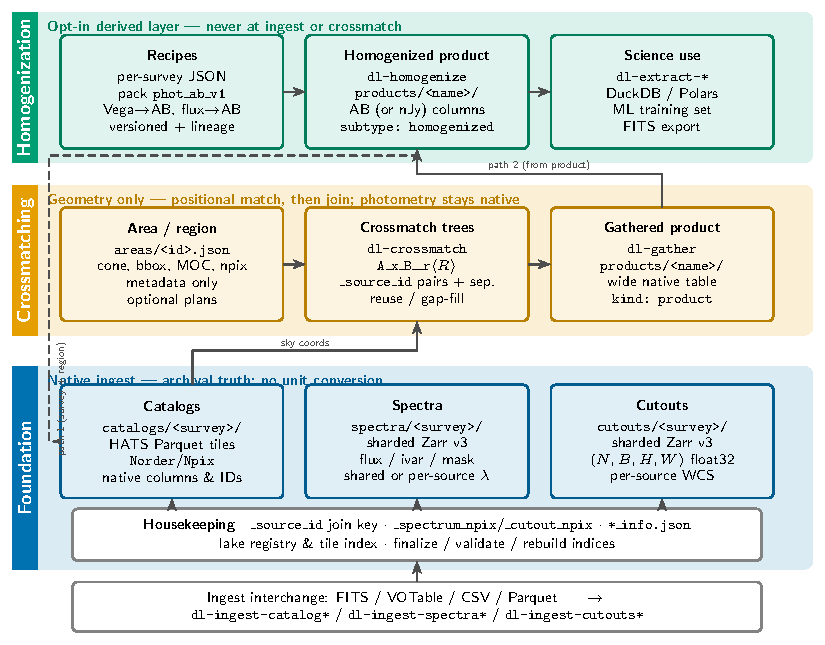
\includegraphics[width=\textwidth]{architecture_layers}
%     \caption{Layered architecture of the astronomy data lake.
%       Native survey data are ingested onto HATS/HEALPix tiles with
%       lake housekeeping (bottom). Positional crossmatch and gather
%       join surveys without changing photometric systems (middle).
%       Homogenization is an opt-in derived product (top). Path~1
%       homogenizes a single survey in a region; path~2 homogenizes a
%       gathered multi-survey product.}
%     \label{fig:lake-architecture}
%   \end{figure*}
%
% Colour mapping (Okabe--Ito, print- and colourblind-safe):
%   blue   = foundation (native ingest)
%   orange = crossmatch + gather (geometry / join)
%   green  = homogenization (opt-in derived products)

\documentclass[tikz,border=6pt]{standalone}

\usepackage{tikz}
\usetikzlibrary{arrows.meta,calc,positioning,backgrounds}

\definecolor{oiBlue}{HTML}{0072B2}
\definecolor{oiOrange}{HTML}{E69F00}
\definecolor{oiGreen}{HTML}{009E73}
\definecolor{oiGrey}{HTML}{4D4D4D}

\begin{document}
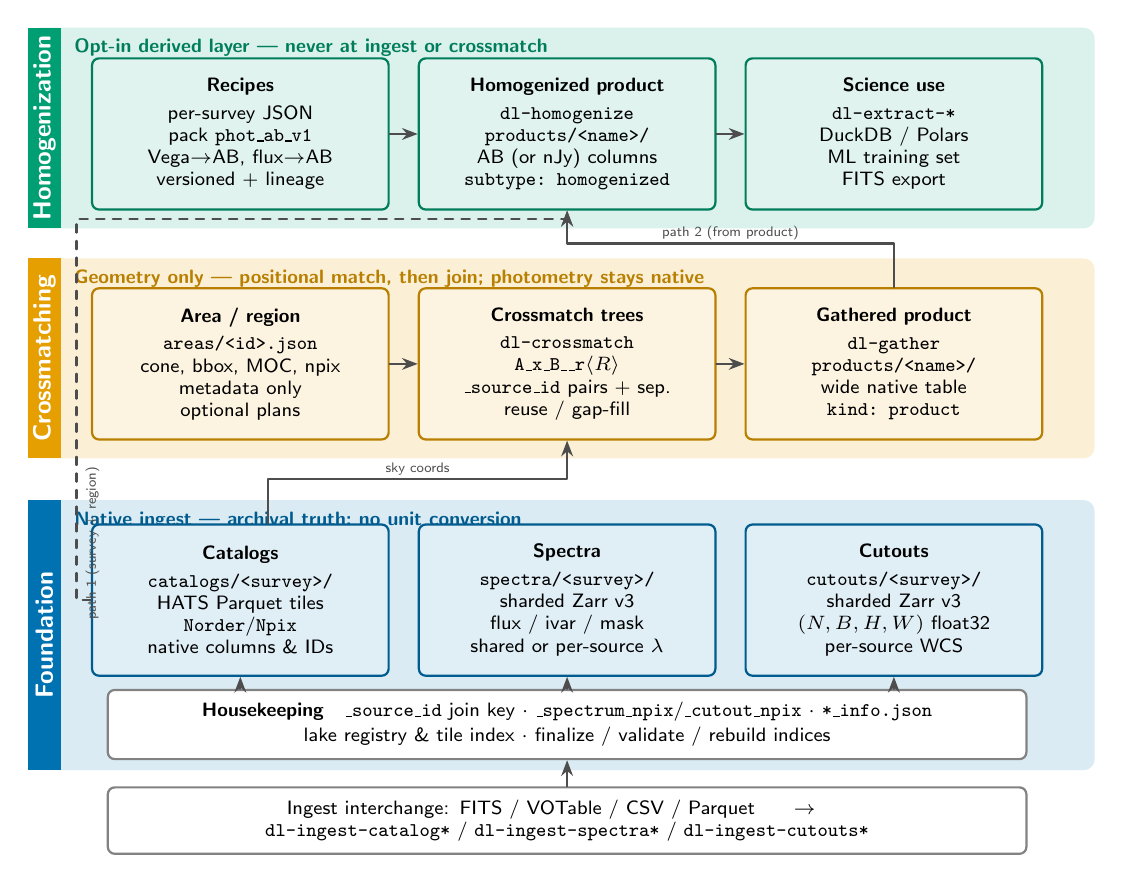
\begin{tikzpicture}[
  font=\sffamily\scriptsize,
  >=Stealth,
  line cap=round,
  line join=round,
  every node/.style={align=center},
  box/.style={
    draw=#1!80!black,
    fill=#1!12,
    thick,
    rounded corners=2.5pt,
    inner sep=4.5pt,
    text width=3.45cm,
    minimum height=1.92cm,
    font=\sffamily\scriptsize
  },
  housebox/.style={
    draw=oiGrey!70,
    fill=white,
    thick,
    rounded corners=2.5pt,
    inner sep=4.5pt,
    text width=11.35cm,
    font=\sffamily\scriptsize
  },
  layerlabel/.style={
    font=\sffamily\bfseries\small,
    rotate=90,
    anchor=center,
    text=white,
    inner sep=2pt
  },
  layerhead/.style={
    font=\sffamily\scriptsize\bfseries,
    inner sep=1pt
  },
  arr/.style={-{Stealth[length=2.0mm]}, thick, oiGrey},
  arrd/.style={-{Stealth[length=2.0mm]}, thick, dashed, oiGrey},
]

% Band geometry (cm). Gaps between bands carry the inter-layer arrows.
\def\W{13.55}
\def\yF{0.12}     % foundation bottom
\def\yFt{3.55}    % foundation top
\def\yC{4.08}     % crossmatch bottom
\def\yCt{6.62}    % crossmatch top
\def\yH{7.00}     % homogenize bottom
\def\yHt{9.55}    % homogenize top
\def\gapCF{3.815} % foundation <-> crossmatch arrow lane
\def\gapHC{6.81}  % crossmatch <-> homogenize arrow lane
\def\gutterx{0.62} % path-1 gutter x
\def\laneoney{7.12} % path-1 horizontal under green boxes

\begin{scope}[on background layer]
  \fill[oiBlue!14, rounded corners=4pt] (0,\yF) rectangle (\W,\yFt);
  \fill[oiOrange!16, rounded corners=4pt] (0,\yC) rectangle (\W,\yCt);
  \fill[oiGreen!14, rounded corners=4pt] (0,\yH) rectangle (\W,\yHt);
  \fill[oiBlue] (0,\yF) rectangle (0.42,\yFt);
  \fill[oiOrange] (0,\yC) rectangle (0.42,\yCt);
  \fill[oiGreen] (0,\yH) rectangle (0.42,\yHt);
\end{scope}

\node[layerlabel] at (0.21,{0.5*(\yF+\yFt)}) {Foundation};
\node[layerlabel] at (0.21,{0.5*(\yC+\yCt)}) {Crossmatching};
\node[layerlabel] at (0.21,{0.5*(\yH+\yHt)}) {Homogenization};

% Column centres (leave a left gutter for the path-1 dashed rail)
\def\cx{2.70}
\def\mx{6.85}
\def\rx{11.00}

% ----- Foundation -----
\node[layerhead, text=oiBlue!80!black, anchor=west]
  at (0.55,\yFt-0.26) {Native ingest --- archival truth; no unit conversion};

\node[box=oiBlue] (cat) at (\cx,2.28)
  {\textbf{Catalogs}\\[2pt]
   \texttt{catalogs/<survey>/}\\
   HATS Parquet tiles\\
   \texttt{Norder}/\texttt{Npix}\\
   native columns \& IDs};

\node[box=oiBlue] (spec) at (\mx,2.28)
  {\textbf{Spectra}\\[2pt]
   \texttt{spectra/<survey>/}\\
   sharded Zarr v3\\
   flux / ivar / mask\\
   shared or per-source $\lambda$};

\node[box=oiBlue] (cut) at (\rx,2.28)
  {\textbf{Cutouts}\\[2pt]
   \texttt{cutouts/<survey>/}\\
   sharded Zarr v3\\
   $(N,B,H,W)$ float32\\
   per-source WCS};

\node[housebox] (house) at (\mx,0.70)
  {\textbf{Housekeeping}\quad
   \texttt{\_source\_id} join key $\cdot$
   \texttt{\_spectrum\_npix}/\texttt{\_cutout\_npix} $\cdot$
   \texttt{*\_info.json}\\[1pt]
   lake registry \& tile index $\cdot$
   finalize / validate / rebuild indices};

% ----- Crossmatching -----
\node[layerhead, text=oiOrange!80!black, anchor=west]
  at (0.55,\yCt-0.26) {Geometry only --- positional match, then join; photometry stays native};

\node[box=oiOrange] (area) at (\cx,5.28)
  {\textbf{Area / region}\\[2pt]
   \texttt{areas/<id>.json}\\
   cone, bbox, MOC, npix\\
   metadata only\\
   optional plans};

\node[box=oiOrange] (xm) at (\mx,5.28)
  {\textbf{Crossmatch trees}\\[2pt]
   \texttt{dl-crossmatch}\\
   \texttt{A\_x\_B\_\_r}$\langle R\rangle$\\
   \texttt{\_source\_id} pairs + sep.\\
   reuse / gap-fill};

\node[box=oiOrange] (gath) at (\rx,5.28)
  {\textbf{Gathered product}\\[2pt]
   \texttt{dl-gather}\\
   \texttt{products/<name>/}\\
   wide native table\\
   \texttt{kind: product}};

% ----- Homogenization -----
\node[layerhead, text=oiGreen!80!black, anchor=west]
  at (0.55,\yHt-0.26) {Opt-in derived layer --- never at ingest or crossmatch};

\node[box=oiGreen] (rec) at (\cx,8.20)
  {\textbf{Recipes}\\[2pt]
   per-survey JSON\\
   pack \texttt{phot\_ab\_v1}\\
   Vega$\to$AB, flux$\to$AB\\
   versioned + lineage};

\node[box=oiGreen] (hom) at (\mx,8.20)
  {\textbf{Homogenized product}\\[2pt]
   \texttt{dl-homogenize}\\
   \texttt{products/<name>/}\\
   AB (or nJy) columns\\
   \texttt{subtype: homogenized}};

\node[box=oiGreen] (use) at (\rx,8.20)
  {\textbf{Science use}\\[2pt]
   \texttt{dl-extract-*}\\
   DuckDB / Polars\\
   ML training set\\
   FITS export};

% ----- Ingest interchange -----
\node[housebox] (raw) at (\mx,-0.52)
  {Ingest interchange: FITS / VOTable / CSV / Parquet
   $\;\rightarrow\;$
   \texttt{dl-ingest-catalog*} / \texttt{dl-ingest-spectra*} / \texttt{dl-ingest-cutouts*}};

% ========== arrows ==========
% ingest -> foundation tiles
\draw[arr] (raw) -- (house);
\draw[arr] (house.north -| cat) -- (cat.south);
\draw[arr] (house.north -| spec) -- (spec.south);
\draw[arr] (house.north -| cut) -- (cut.south);

% catalog sky coordinates -> crossmatch (lane between bands; offset so it
% does not look like Catalogs -> Area)
\draw[arr] ([xshift=10pt]cat.north) -- ([xshift=10pt]cat.north |- 0,\gapCF)
  -- node[above, font=\sffamily\tiny, text=oiGrey, inner sep=1pt] {sky coords}
     (xm.south |- 0,\gapCF) -- (xm.south);

% area plan -> match -> gather
\draw[arr] (area) -- (xm);
\draw[arr] (xm) -- (gath);

% path 2: gathered native product -> homogenize (lane between bands)
\draw[arr] (gath.north) -- (gath.north |- 0,\gapHC)
  -- node[above, font=\sffamily\tiny, text=oiGrey, inner sep=1pt] {path 2 (from product)}
     (hom.south |- 0,\gapHC) -- (hom.south);

% path 1: single survey + region, skip crossmatch/gather.
% Up the left gutter, then under the green boxes into homogenize.
\draw[arrd] (cat.west) -- (\gutterx,2.28) -- (\gutterx,\laneoney)
  -- (hom.south |- 0,\laneoney) -- (hom.south);
\node[font=\sffamily\tiny, text=oiGrey, rotate=90, anchor=center]
  at (0.82,3.0) {path 1 (survey + region)};

% recipes -> product -> science
\draw[arr] (rec) -- (hom);
\draw[arr] (hom) -- (use);

\end{tikzpicture}
\end{document}
